\begin{figure}[H]
\begin{center}
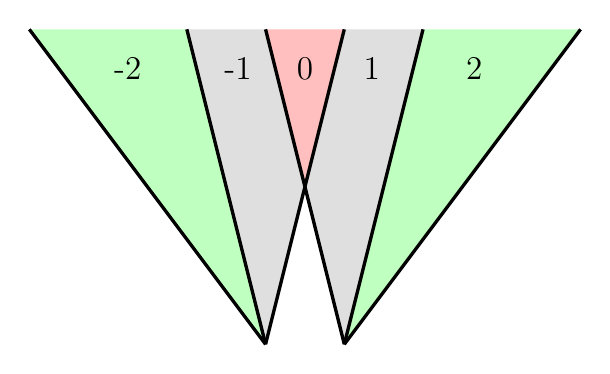
\begin{tikzpicture}
\fill[fill=gray!25] (8,0) -- (8.5,2) -- (8,4) -- (7,4) -- (8,0); % Left block (center)
\fill[fill=gray!25] (9,0) -- (8.5,2) -- (9,4) -- (10,4) -- (9,0); % Right block (center)
\fill[fill=red!25] (8.5,2) -- (8,4) -- (9,4) -- (8.5,2); % Center block
\fill[fill=green!25] (8,0) -- (5,4) -- (7,4) -- (8,0); % Left block
\fill[fill=green!25] (9,0) -- (12,4) -- (10,4) -- (9,0); % Right block
\draw[very thick] (9,0) -- (8,4);
\draw[very thick] (9,0) -- (10,4);
\draw[very thick] (9,0) -- (12,4);
\draw[very thick] (8,0) -- (9,4);
\draw[very thick] (8,0) -- (7,4);
\draw[very thick] (8,0) -- (5,4);
\node at (6.25,3.5) {\large-2};
\node at (7.65, 3.5) {\large-1};
\node at (8.5, 3.5) {\large0};
\node at (9.35, 3.5) {\large1};
\node at (10.65, 3.5) {\large2};
\end{tikzpicture}
\caption{Combined field of view.}
\label{sensarea1}
\end{center}
\end{figure}